\documentclass[a4paper, 12pt]{article}
\usepackage[utf8]{inputenc}
\usepackage[portuguese]{babel}

\usepackage{mathptmx}
\usepackage{enumitem}
\usepackage{amsmath,amssymb,exscale}
\usepackage{textcomp}

\usepackage{multirow}

% Margins
\usepackage{geometry}
\geometry{left=30mm,right=20mm,%
bindingoffset=0mm, top=30mm,bottom=20mm,includefoot}

% Images
\usepackage{graphicx}
\graphicspath{ {./images/} }

% Title font size
\usepackage{titlesec}
\titleformat*{\section}{\bfseries}

% Indent first sentence of a paragraph
\usepackage{indentfirst}

% Page numbers at bottom right
\usepackage{fancyhdr}
\pagestyle{fancy}
\fancyhf{}
\renewcommand{\headrulewidth}{0pt}
\rfoot{\thepage}

% 1.5 line spacing (yes, 1.25 is actually 1.5)
\fontsize{10}{12}
\linespread{1.50}
\fontfamily{ptm}
\selectfont

% Fix vspacing for section titles
\let\oldsection\section
\renewcommand{\section}[1]{{\vspace{20pt}\oldsection*{#1}\vspace{-10pt}}}

% Indent size
\setlength\parindent{10mm}

% Jump 20pt
\newcommand{\jump}[1]{{\vspace{20pt}}}

\newenvironment{leftquote}[1][]
{
    \hspace{30pt} #1
    \vspace{20pt}
    \fontsize{10}{10}\selectfont
    \begin{flushright}
    \begin{minipage}{120mm}
}
{
    \end{minipage}
    \end{flushright}
    \par
    \vspace{20pt}
}

\newcommand{\tmp}{}

\newenvironment{container}[3]
{
    \renewcommand{\tmp}{#3} %gambiarra
    
    \begin{center}
    \begin{minipage}{#1}
    \centering
    #2
}
{
    \raggedright
    {\footnotesize \tmp}
    \end{minipage}
    \end{center}
}

\usepackage{listings}
\usepackage{amsmath,amssymb,caption}
%% my poor man's solution to arc notation
\newcommand{\tarc}{\mbox{\large$\frown$}}
\newcommand{\arc}[1]{\stackrel{\tarc}{#1}}

\lstset{frame=tb,
  language=Matlab,
  aboveskip=3mm,
  belowskip=3mm,
  showstringspaces=false,
  columns=flexible,
  basicstyle={\small\ttfamily},
  numbers=none,
  numberstyle=\tiny\color{gray},
  keywordstyle=\color{blue},
  commentstyle=\color{dkgreen},
  stringstyle=\color{mauve},
  breaklines=true,
  breakatwhitespace=true,
  tabsize=3
}

\begin{document}

% Remove page number
\clearpage
\thispagestyle{empty}

\begin{bfseries}
\begin{center}


\includegraphics{ufc.png} \\
\vspace{-4pt} 
UNIVERSIDADE FEDERAL DO CEARÁ \\
\vspace{4pt} 
CENTRO DE TECNOLOGIA \\
\vspace{4pt} 
DEPARTAMENTO DE ENGENHARIA DE TELEINFORMÁTICA \\
\vspace{4pt}
ELETROMAGNETISMO APLICADO \\
\vspace{4pt}
SEMESTRE 2024.1 \\


\vspace*{\fill}
\textbf{ATIVIDADE 01}
\vspace*{\fill}

\end{center}

\begin{itemize}[leftmargin=*]
    \setlength{\itemsep}{0pt}
    \item[] ALUNO: Ruan Pereira Alves
    \item[] MATRÍCULA: 569551
    \item[] PROFESSOR: João Batista
    \item[] DISCIPLINA: Eletromagnetismo Aplicado
    \item[] DATA DE ENTREGA DO RELATÓRIO: 18/04/2024
\end{itemize}

\end{bfseries}

\newpage

\section{QUESTÕES}

\textbf{Questão 01} 

a) V = $3x^2 + xz$

O cálculo é realizado de acordo com a operação da biblioteca Sympy, uma biblioteca de matemática simbólica. Definindo a equação e os símbolos a serem utilizados, bem como o tipo de coordenadas a serem utilizadas em cada questão, a biblioteca é capaz de realizar os cálculos bem como dito no livro texto da disciplina.

Para realizar os cálculos do item A, primeiro foi definido quais seriam as coordenadas utilizadas (mais informações no próprio código, com os comentários). 

Após a definição do campo, a função de gradiente foi executada, trazendo o primeiro resultado da forma como mostrado no livro-texto Eletromagnetismo, Hayt 8° edição, capítulo 4, seção 6, na página 94, 
a partir dos cálculos de derivadas parciais, que pode ser visto abaixo: 

\begin{figure}[!h]
	\centering
	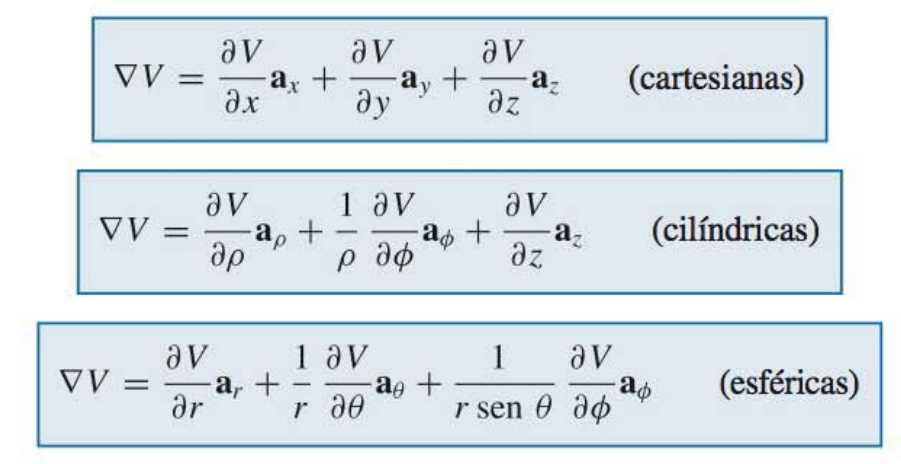
\includegraphics[scale= 0.6]{images/gradiente.png}
	\caption{Definição do cálculo do gradiente de acordo com cada sistema de coordenadas. Fonte: Próprio Autor}
\end{figure}

Dado que o cálculo do laplaciano pode ser dado como sendo o divergente de um gradiente, foi feita dessa forma os cálculos de laplacianos. O cálculo do divergente na biblioteca também é de acordo com a definição matemática, como mostrado no livro texto: 

\begin{figure}[!h]
	\centering
	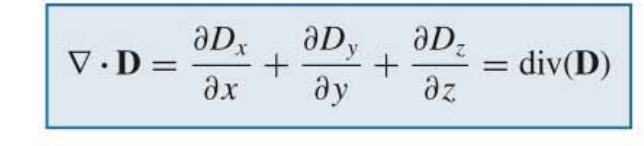
\includegraphics[scale= 0.6]{images/divergente.png}
	\caption{Definição do cálculo do divergente. Fonte: Próprio Autor}
\end{figure}

Para o rotacional, também foi seguido o mesmo padrão e rigor matemático da biblioteca, e dado o fato de que o rotacional do gradiente de um campo vetorial é 0, dado as propriedades feitas a partir do Teorema da Divergência, como dito em sala de aula. Também é possível observar isso no livro Classical Electrodynamics, do autor John David Jackson e no Elementos do Eletromagnetismo, do Sadiku. 

\begin{figure}[!h]
	\centering
	
\includegraphics[scale= 0.6]{images/rotacional.png}
	\caption{Propriedade do rotacional segundo David Jackson. Fonte: Próprio Autor}
\end{figure}

\begin{figure}[!h]
	\centering
	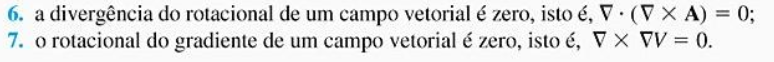
\includegraphics[scale= 0.6]{images/rotacional1.png}
	\caption{Propriedade do rotacional segundo Sadiku. Fonte: Próprio Autor}
\end{figure}

O mesmo processo foi seguido para os items b) e c). Sendo assim, temos como resultado: 

\begin{figure}[!h]
	\centering
	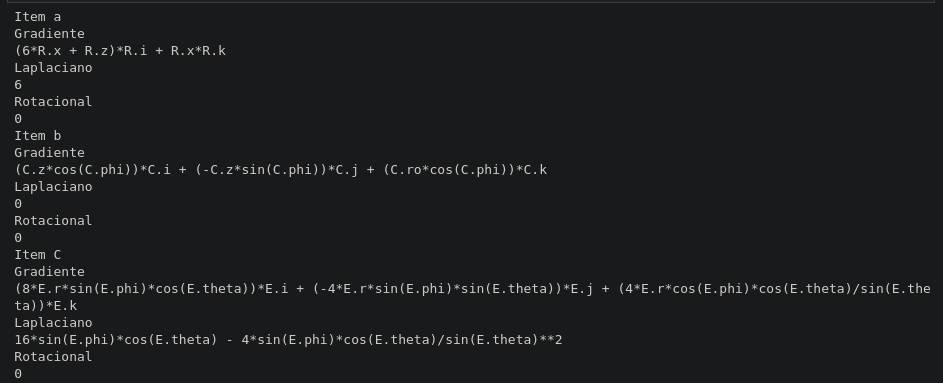
\includegraphics[scale= 0.6]{images/questão01.png}
	\caption{Resultados computacionais da Questão 1. Fonte: Próprio Autor}
\end{figure}

\textbf{Questão 02}

\textbf{Questão 03}

\textbf{Questão 04}

\textbf{Questão 05}

Temos que, segundo o livro texto Hayt, capítulo 4, seção 6, página 92, que a intensidade do campo elétrico a partir do potencial é dado por: 

\begin{figure}[!h]
	\centering
	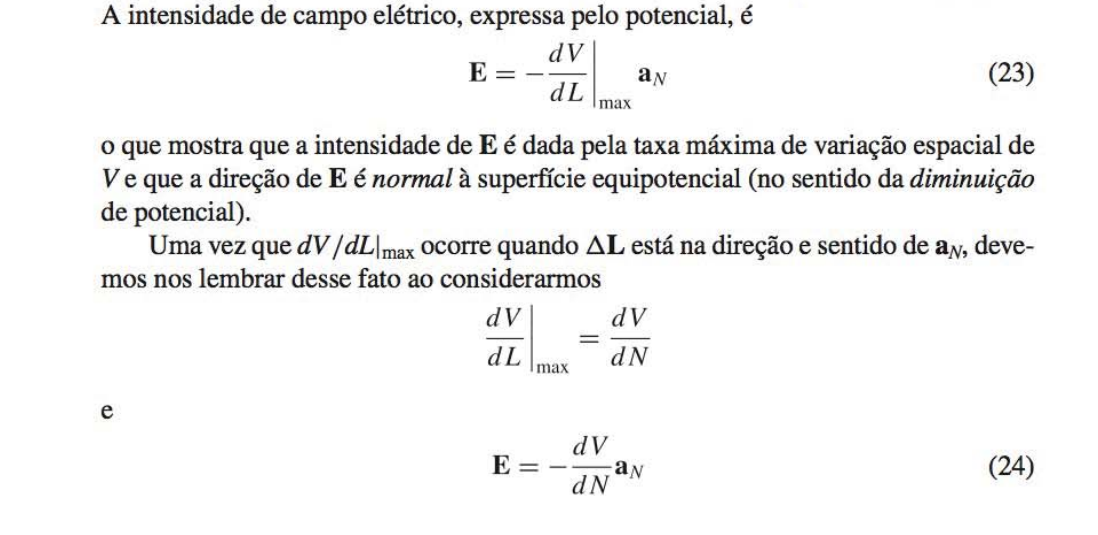
\includegraphics[scale= 0.6]{images/intensidade1.png}
	\caption{Definição da intensidade do campo elétrico a partir do potencial. Fonte: Próprio Autor}
\end{figure}

Mas temos apenas o desenvolvimento em x. Logo, ficamos com 

\begin{equation}
	E = - \frac{dV}{dX}* \mathbf{a}_X
\end{equation}

A partir disso, temos os resultados a seguir:

Para o item A:

\begin{figure}[!h]
	\centering
	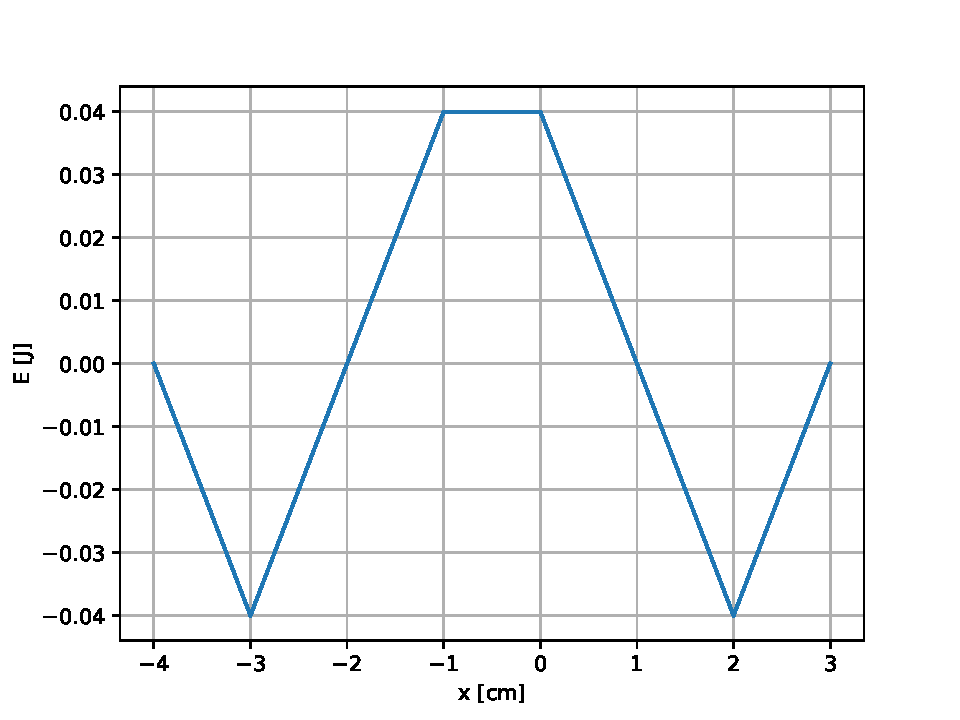
\includegraphics[scale= 0.6]{images/q5a.pdf}
	\caption{Item A. Fonte: Próprio Autor}
\end{figure}

\newpage

Para o item B:

\begin{figure}[!h]
	\centering
	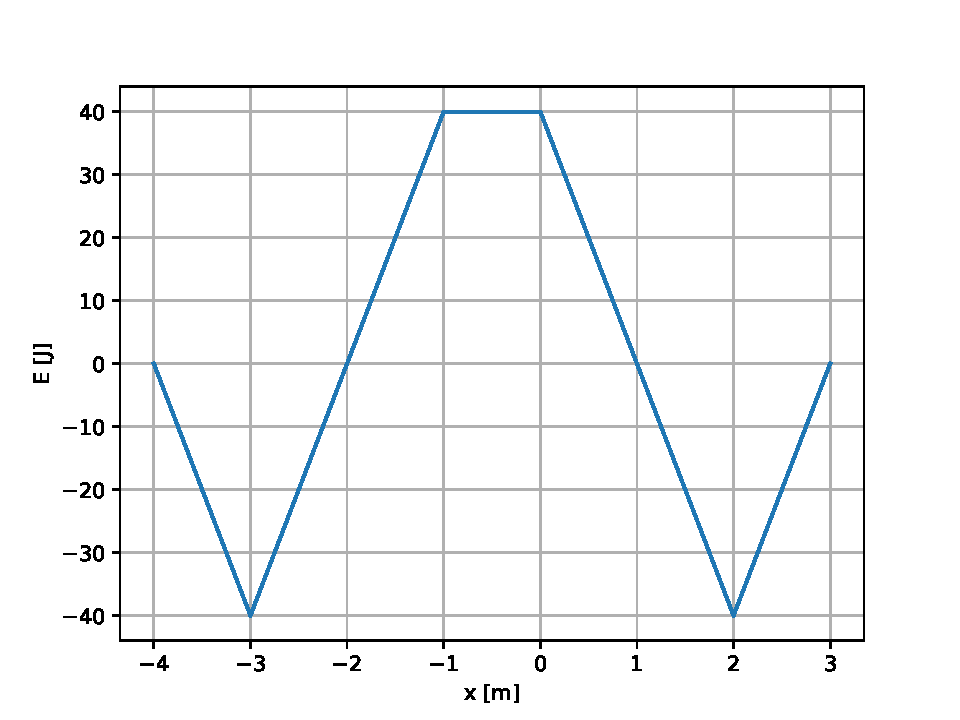
\includegraphics[scale= 0.6]{images/q5b.pdf}
	\caption{Item B. Fonte: Próprio Autor}
\end{figure}


\end{document}